\chapter{\sffamily Simple state transitions}

{\bfseries\sffamily Concept.} To define and develop an archetype simulation environment for simple state transitions. In our classification scheme, this archetype is defined by a trivial state partition graph topology and would make sense for simulations of sequential design problems, sports matches and other simple gameplay domains. In this chapter we will discuss the typical ways in which the state of the system may only partially be observed in realistic examples, and analyse how best to deal with each situation. For the mathematically-inclined, this chapter will define the mapping of our formalism to simple state transitions. For the programmers, the software which is designed and described in this chapter can be found in the public Git respository here: \href{https://github.com/worldsoop/worldsoop}{https://github.com/worldsoop/worldsoop}.


\begin{figure}[h]
\centering
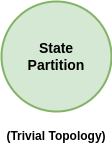
\includegraphics[width=2cm]{images/chapter-6-state-partition-graph.drawio.png}
\caption{State partition graph topology for simple state transition archetypes.}
\label{fig:state-partition-graph-simple-state-transitions}
\end{figure}
